\section{Observations}
\label{sec:observations}

\begin{figure*}[t]
  \centering
  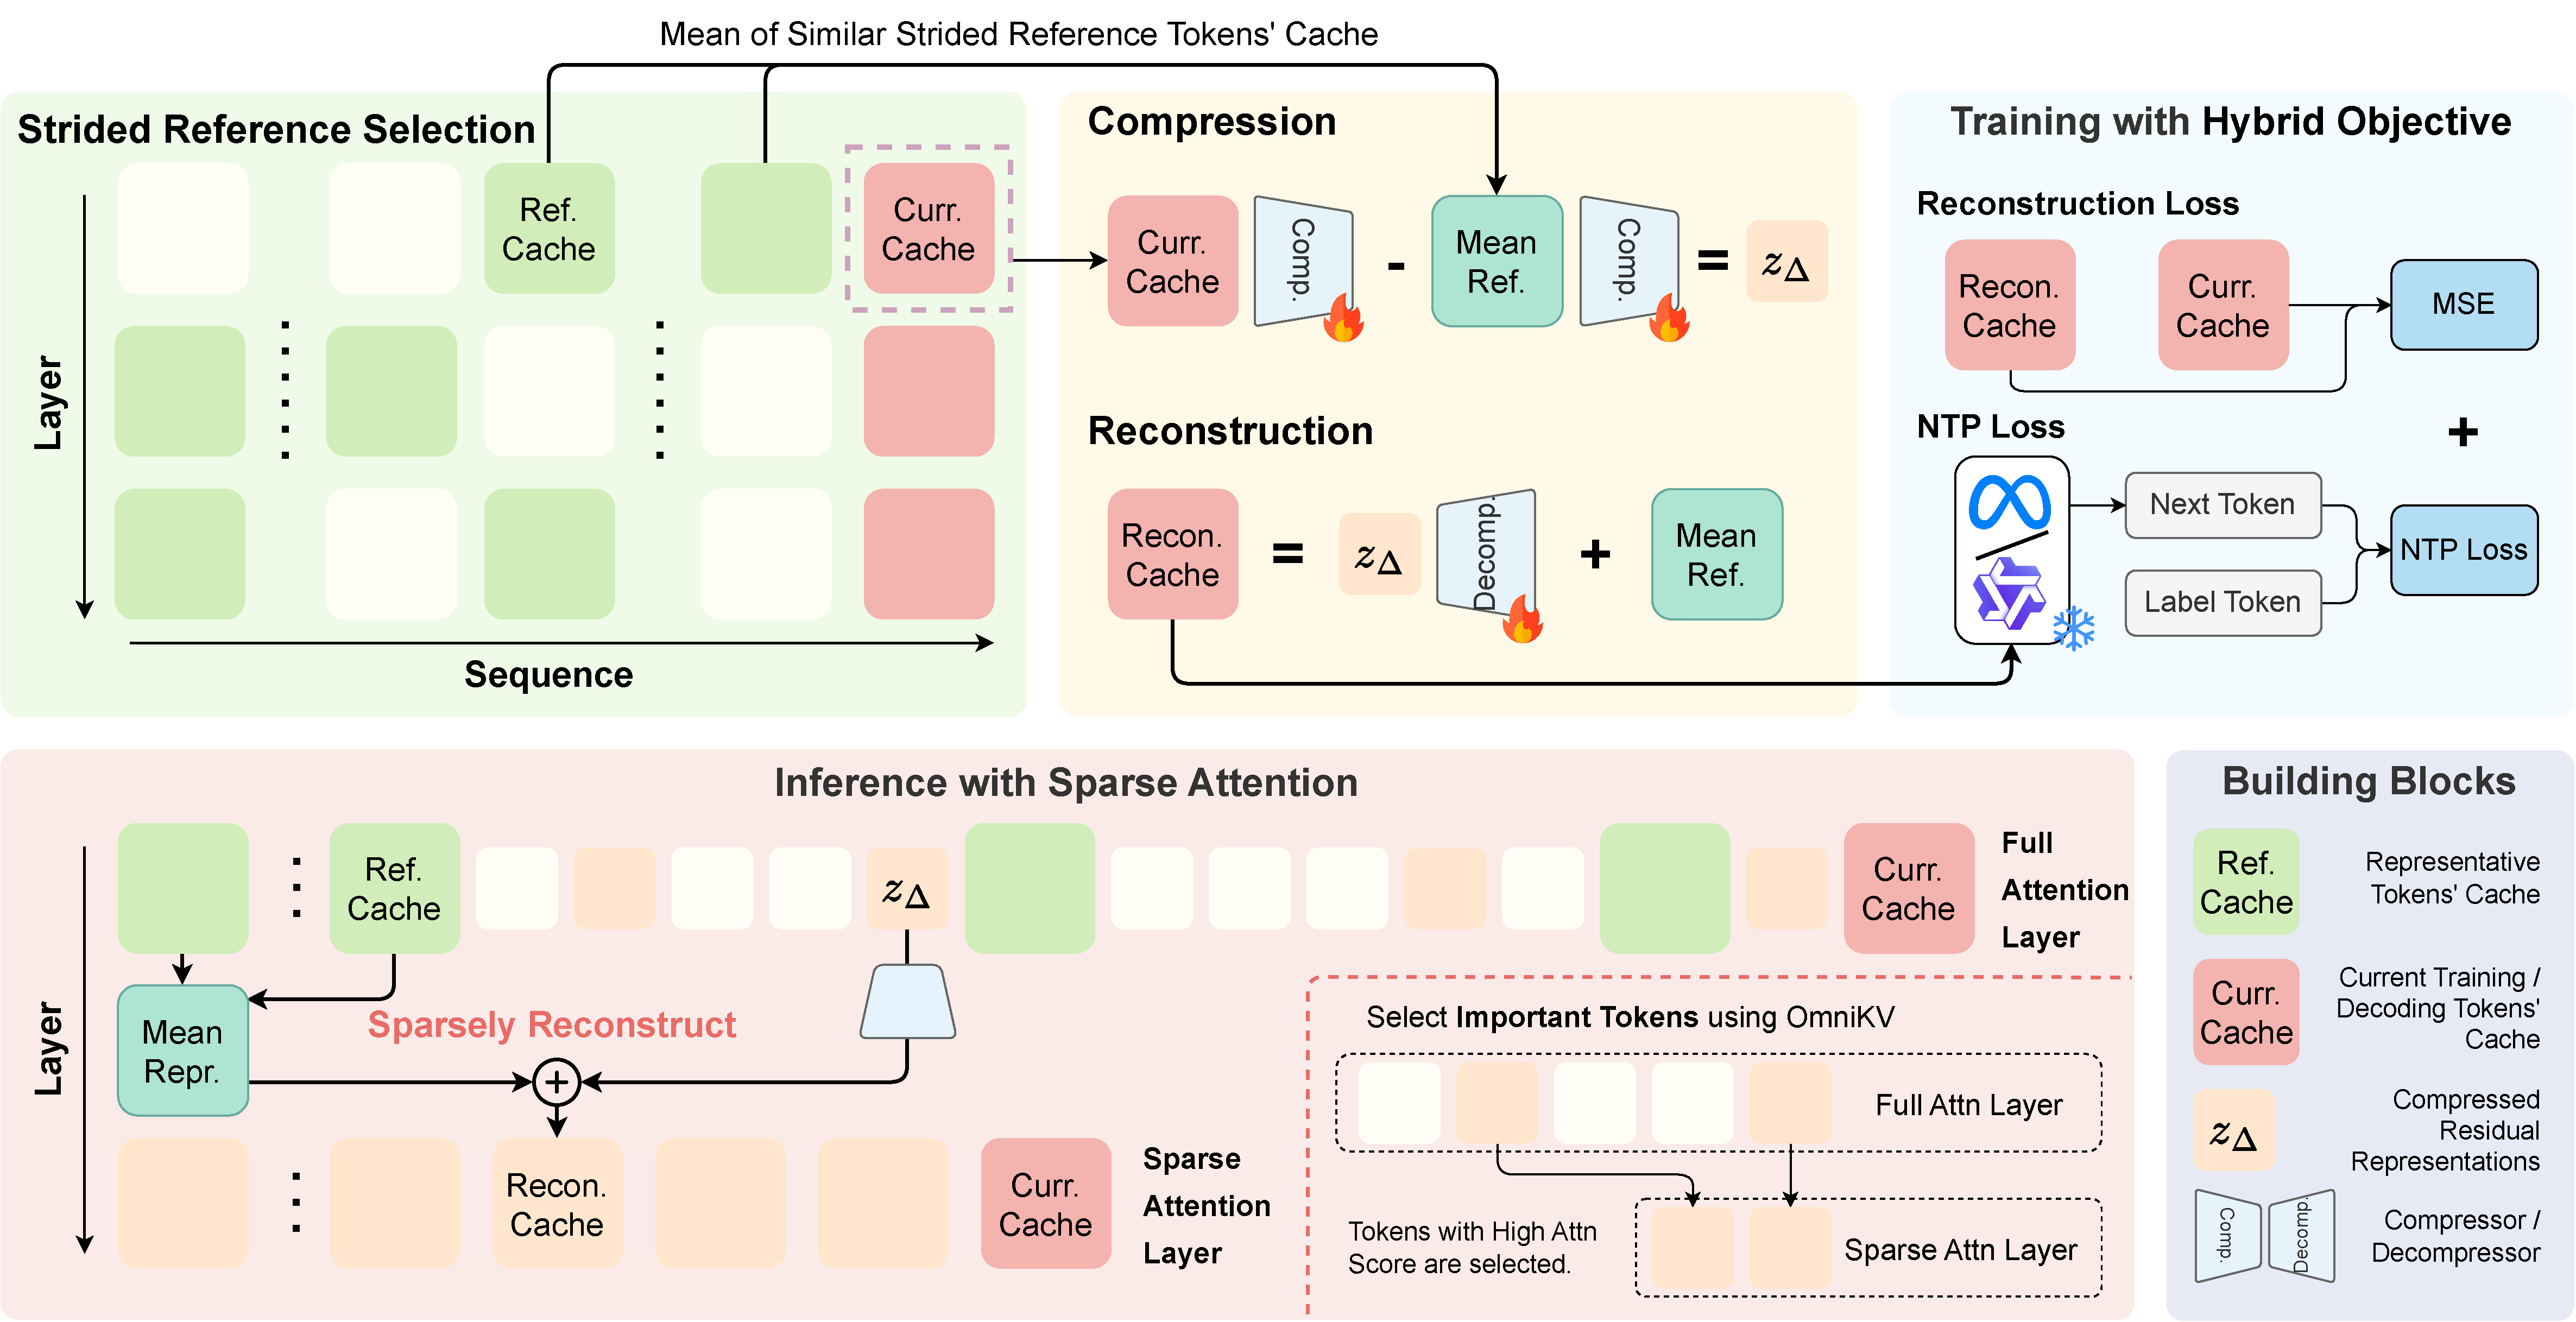
\includegraphics[width=0.99\textwidth]{figures/DeltaKV-framework.pdf} 
  \caption{\textbf{Overview of DeltaKV.} 
  DeltaKV compresses KV caches by encoding token-wise residuals relative to globally retrieved reference tokens, trained with a hybrid MSE+NTP objective (top).
  At inference, DeltaKV integrates with sparse attention (e.g., OmniKV), storing compressed residuals and reconstructing only selected tokens on demand, reducing memory usage while preserving accuracy (bottom).} 
  \label{fig:DeltaKV}
  \vspace{-1.0em}
\end{figure*}

\vspace{-0.25em}
\paragraph{Background and Notation}
DeltaKV targets standard Transformer architectures such as Qwen~\cite{yang2025qwen2_1m} and Llama~\cite{grattafiori2024llama3}. Each layer consists of self-attention and a feed-forward network (FFN).
%%%
Let $\Wq \in \mbb{R}^{d_\mrm{q}\times d}$, $\Wk \in \mbb{R}^{d_\mrm{k}\times d}$, $\Wv \in \mbb{R}^{d_\mrm{v}\times d}$, and $\Wo \in \mbb{R}^{d\times d}$ be the query, key, value, and output projections, where $d$ is the hidden size, and $d_\mrm{q}, d_\mrm{k}, d_\mrm{v}$ denote the total query/key/value dimensions across heads. 
Generally, $d_\mathrm{k} = d_\mathrm{v}$.

During inference, the KV cache stores key-value states (i.e., $\bm{K}, \bm{V}$) from previous tokens to avoid recomputation.
Given token embeddings $\bm{H} \in \mathbb{R}^{B\times L\times d}$, the KV cache is computed as $\bm{K}=\bm{H}\Wk$ and $\bm{V}=\bm{H}\Wv$, both with shape $[B, L, d_\mathrm{k}]$ or equivalently $[B, L, N, D]$, where $B$ denotes the batch size, $N$ the number of key/value heads, $L$ the sequence length, and $D$ the key/value head dimension. 

Inference consists of a \emph{prefill} phase that constructs the KV cache and an autoregressive \emph{decode} phase.
%%%
For long contexts, \emph{chunk prefill} reduces activation memory without altering the computation.
%%%
To analyze KV cache redundancy, we define the \textbf{Residual KV} as: 
\vspace{-0.25em}
\begin{displaymath}
  \bm{KV}_\Delta=\bm{KV}-\overline{\bm{KV}}_R,
  \vspace{-0.25em}
\end{displaymath}
where $\bm{KV} = \mathrm{Concat}(\bm{K}, \bm{V})$ and $\overline{\bm{KV}}_R$ is the mean of the $k$ nearest historical \emph{reference} tokens. 
%%%
All analyses are conducted on Qwen2.5-7B-Instruct-1M \cite{yang2025qwen2_1m}. The results are presented in Figure \ref{fig:combined_analysis_results}.


\paragraph{Observation 1: \emph{Long-Range} Inter-Token Similarity}
Token redundancy in natural language is not confined to local neighborhoods. 
While prior work like CacheGen~\cite{liu2024cachegen} emphasizes locality (similarity to immediate neighbors), we find that a token’s closest semantic match often lies far back in the context.
%%%
As shown in Figure \ref{fig:token_sim_dist}, KV representations frequently exhibit cosine similarity above \textbf{0.9} with historical tokens. 
More strikingly, Figure~\ref{fig:distance_dist_to_sim_tokens} shows that over \textbf{60\%} of the most similar tokens occur at distances greater than 16.
%%%
This pervasive \emph{long-range} similarity indicates that effective KV compression must leverage global retrieval rather than local heuristics.

\paragraph{Observation 2: \emph{Highly Shared} Latent Components}
We further observe that KV caches share dominant high-norm latent directions, reflecting common linguistic and structural patterns.
SVD analysis (Figure~\ref{fig:svd_analysis_of_token_cache}) reveals a steep spectral decay in original KV representations, whereas residual KV exhibits a significantly flatter spectrum.
%%%
Subtracting retrieved references effectively removes these shared components. As a result, residual KVs collapse to low-magnitude, noise-like signals: their L2 norms shrink substantially (Figure~\ref{fig:l2_norm_dist_gap}), and their value distribution becomes sharply concentrated around zero (Figure~\ref{fig:residual_kv_range_dist}).
%%%
This suggests that most KV cache capacity is consumed by redundant shared structure, while token-specific information is both low-energy and inherently easier to compress.
